\section{Design and Implementation}
\label{sec:implementation}

This section discusses the implementation and design of \MP{} on profiling different aspects of an allocator. 
%To profile an allocator, \MP{} intercepts memory allocations/deallocations, memory-related system calls, and synchronizations. This also indicates that an allocator should utilize standard APIs in order for \MP{} to collect corresponding information. However, the Linux allocator utilizes the internal implementation of synchronizations by default. For the profiling purpose, it should be changed to invoke explicit POSIX-APIs instead. Fortunately, most allocators do not need any change or the recompilation.  \MP{} profiles the performance, memory overhead, scalability, and application friendliness, as discussed in different subsections. 

 %It also discusses some common issues, such as adapting to different allocators, and the performance issue of collecting data. 

\subsection{Profiling Performance Data}

\label{sec:performanceimplement}

\MP{} measures the average time of every memory management operation, such as allocations and deallocations, which is the important metrics to evaluate an allocator. The RDTSC instruction is employed to collect the time due to its accuracy and low overhead. Basically, \MP{} intercepts all allocation invocations, such as \texttt{malloc}, \texttt{calloc}, and \texttt{realloc}, and memory deallocations, such as \texttt{free}, and collects the time before and after each operation. The difference between them is the runtime of this operation.  

% How to differentiate based the type? How to verify whether this a new/re-used allocation (efficiently)? 
Since an allocator typically has different execution paths for different types of objects, such as new or re-used allocations of small objects, or allocation of big objects, \MP{} further collects the information for each type separately. Note that some allocators, such as Hoard, even have a different execution path for objects with medium sizes, between 256 bytes and 8K bytes. Based on our evaluation, the average allocation time for small and big objects can be as large as orders of magnitude. The fine-grained data helps identify design issues for a specific type. \MP{} differentiates the types of allocations and deallocations by checking the requested size with the threshold stored in the configuration file (as described in Section~\ref{sec:understandingallocators}). In order to differentiate new allocations from re-used allocations, with over $3\times$ performance difference, \MP{} utilizes a global hash table to track objects: every allocated object will be inserted into the hash table in its allocation time, and will be kept in the table; If an allocation is found to be in the hash table, then this allocation is a re-used allocation. Otherwise, it is a new allocation. 

\MP{} also differentiates operations for the serial and parallel phase. In the serial phase, there is just one thread, typically just the main thread. But there are multiple threads in parallel phase, as its name implies. The operation of the parallel phase may require more than $2\times$ of time than that in serial phase, mainly caused by user-space or kernel space contention. \MP{} excludes the time for the first allocation, since many allocators will perform its initialization upon the first allocation.  

% How to use sampling mechanism to further reduce the overhead? 
\MP{} also employs PMUs to collect hardware events upon each memory operation, such as cache misses, page faults, and instructions. These hardware events are significant supplements for identifying an issue, given that \MP{} is a non-intrusive profiler that cannot know the implementation details of an allocator. For instance, DieHarder is generally very slow, which often has an unusual number of cache misses for each deallocation. With the events of cache misses, we could identify a design issue of DieHarder: it traverses all memory bags one by one to determine the original bag for an object, causing an excessive number of cache misses. Similarly, \MP{} collects hardware events before and after each operation, and uses the difference of two counters as the number of events occurring inside an operation. The Linux kernel has supported PMUs starting from 2009 (Linux-2.6.31)~\cite{pmulinuxsupport}, where users could set up performance monitoring via the \texttt{perf\_event\_open} system call. However, the collection of hardware events is still the most expensive operation in \MP{}, which will incur more than $2\times$ slowdown on average if all memory operations will collect such events. Therefore, \MP{} has two methods to reduce its overhead. First, \MP{} only collects hardware events for 1 out of 100 memory operations, which helps reduce the overhead. Second, \MP{} provides an option that allows users to choose this functionality if necessary, since normal users typically do not need to know the implementation details. Therefore, normal users do not have to pay the overhead.     


\subsection{Profiling Memory Overhead}
\label{sec:profilingmemory}

For memory overhead, \MP{} reports the amount and the ratio of different types of memory overhead, such as internal fragmentation, memory blowup, and external fragmentation (and others), and real memory usage, so that programmers can pinpoint the issues of excessive memory consumption. As described in Section~\ref{sec:intro}, \MP{} tracks real memory usage on pages precisely, since the OS will allocate a physical page only when any word of this page is assessed. \MP{} intercepts memory-related system calls in order to obtain the total memory usage. For an allocator, the difference between total and real memory usage is memory overhead, which is the sum of internal fragmentation, memory blowup, and external memory fragmentation. Note that the metadata will be attributed to external fragmentation and others, which cannot be easily separated. However, it is still challenging to measure these memory overhead precisely and efficiently, as discussed in the following. 

For a small object, its internal fragmentation is the difference between its size class and the requested size. However, if the difference is larger than a page, this method will not work. We need to consider allocation policy that the OS always allocates a physical page in a demanding way. For such objects, internal fragmentation should be measured differently: for a new allocation, the internal fragmentation will be difference between the end of the object and the end of its last page; For a re-used object, \MP{} should track the maximum pages of this object, and use the difference between the end of its last page and the end of the object as internal fragmentation. When an object is released, its internal fragmentation should be decremented. \MP{} utilizes the same hash table as described in Section~\ref{sec:performanceimplement} to track the maximum pages for each object. Internal fragmentation for big objects should be measured on the page level as well. \MP{} also tracks memory related system calls, such as \texttt{munmap} and \texttt{madvise}, in order to understand the real physical memory usage.  

It is also challenging to measure memory blowup. By definition, a new allocation will be treated as memory blowup if there exist freed objects for this size class in the freelists of other threads. However, this definition does not specify whether memory blowup should be reduced upon the succeeding deallocation and re-allocation. For instance, the total memory situation can be changed upon next re-allocation. Instead, \MP{} is based on such an observation: \textit{all freed objects of a size class represent the upper bound for its memory blowup; This upper bound subtracted by the size of recently-freed objects will be memory blowup for a size class}. Based on this observation, \MP{} further implements a practical method that uses a global counter to track recently-freed objects for each size class. This global counter is incremented upon every deallocation, but will be decremented upon each allocation if the counter is greater than zero. \MP{} will compute memory blowup for each size class of small objects and for big objects, and then utilizes the summary as the final memory blowup. After getting the memory blowup, \MP{} will compute external memory consumption (and others) that is equal to the subtraction of memory blowup and internal fragmentation from the total memory overhead.

In the end, \MP{} will report memory wastes when memory consumption of an application reaches its maximum value. However, it is very expensive to frequently collect the data of memory wastes. Instead, \MP{} only updates this data, when the total memory usage is increased by 1MB. Also, it is very expensive to update all data frequently using global counters, since this will cause significant cache contention. Therefore, \MP{} tracks most data with thread-local variables, and summarizes all data together when necessary. \MP{} only uses global variables for total memory consumption and counters of recently-freed objects for each size class. 
%However, even with global variables, it is still expensive to update them with the full synchronization or even atomic variables. Instead, \MP{} updates these variables without synchronization, which may lose some updates. However, based on our evaluation, \MP{} should still provide a reliable percentage for different types of memory overhead.  

\subsection{Profiling Scalability}
\label{sec:profilingscale}

\MP{} reports two types of scalability data: one is about locks that indicate user space contention, while the other one is about memory-related system calls that may indicate kernel space contention. Note that \MP{} only focuses on the contention inside memory management operations, which is different from general synchronization profilers~\cite{SyncProf, SyncPerf, wPerf}.

For user-space contention, \MP{} reports the total number of locks, and the number of lock acquisitions, the contention rate, and the average cycle of each lock acquisition and each critical section for each type of memory operation. The contention rate and the number of lock acquisitions per operation are two very important metrics to identify design issues of an allocator, as further described in Section~\ref{sec:effectiveness}.  \MP{} intercepts memory management operations and POSIX synchronizations, but only counts synchronizations inside memory management operations. If an allocator is using non-standard synchronizations, such as atomic variables, \MP{} cannot report user-space contention correctly. In order to collect the average cycles, \MP{} utilizes the RDTSC instruction to collect the runtime of each lock operation. The contending status of a lock acquisition could be easily recognized by the value of a lock. For instance, the non-zero value of $mutex.\_\_data.\_\_lock$ implies that the lock has been acquired by other threads, and therefore is contending. 

% How to determine the contention. 

For kernel-space contention, \MP{} mainly collects the number of invocations and the average runtime of memory-related system calls inside each type of memory management operation, where these system calls include \texttt{mmap}, \texttt{munmap}, \texttt{mremap}, \texttt{sbrk}, \texttt{madvise}, and \texttt{mprotect}. These memory-related system calls  acquire a per-process mmap lock at the entry, same for page fault handler. Therefore, when there is high lock contention inside the kernel, the runtime of every memory-related system call will be excessively larger than that without the contention. For instance, the Linux allocator of \texttt{glibc-2.21} slows down \texttt{dedup} by 27\%, which can be uncovered by the excessive number of \texttt{madvise} system calls and an extremely-high runtime (up to 12266 cycles) of each memory-related system call. The detailed description of this bug can be seen in Section~\ref{sec: benifitdesigners}.  

\subsection{Application Friendliness}
\label{sec:profilefriendliness}

%Currently,

\begin{comment}
Cache line utilization: 
Shadow memory. 
Cache line: real using memory.
page: real used memory.

False sharing: 
Lines:
Cache contention rate: owner, if the current write operation is not the existing owner, we will increment the counter. 
We will report the percentage with write. 

False sharing, 
active/passive: 
how many lines with active and passive. 
	
\end{comment}

 
For application friendliness, \MP{} focuses on whether an allocator is tapped well with memory usage pattern and memory access pattern of an application.  More specifically, \MP{} will report cache/page utilization rate, cache contention rate, false sharing effect, and some hardware related events, which could also significantly impact the performance of applications. 

Cache utilization rate is the average percentage of each cache line that has been used to hold real data. A low cache utilization rate may degrade the performance. For instance, the \texttt{glibc} allocator places metadata just before real objects, which will reduce cache utilization rate since metadata are not used as frequently as real data. Page utilization rate is similar to this, but focusing on the page level instead. In order to collect  utilization rates, we will collect the utilization rate for every memory access, and then compute the average of all accesses. In order to reduce the overhead, \MP{} chooses to sample memory accesses with the hardware PMUs, which will sample one access out of $100,000$ accesses. 

To compute the utilize rate, \MP{} maintains the number of used bytes for each cache line and each page, which will be updated on each allocation and deallocation. We assume that all allocated bytes will be used. In implementation, upon every sampled event, \MP{} increments the number of cache lines and pages that have been accessed, and also increments the counter for used bytes on the current cache line. In the end, \MP{} computes the utilization rate with a simple division. For cache utilization rate, the dividend is the total number of used bytes, and the divisor is the the total number of bytes for these cache lines. The page utilization rate is computed similarly.

However, the challenge is to quickly locate the metadata for each cache line and page, since the metadata should be updated upon every allocation and deallocation, as well as upon every sampled event. During its implementation, \MP{} tried multiple mechanisms. First, \MP{} designed a red-black tree to hold memory mappings of the heap, and then stored the address of corresponding metadata on the tree node. This mechanism was found to be inefficient, as some allocators may include thousands of mappings, which may unfortunately introduce tens of comparisons for each update. Second, \MP{} utilized a hash map to store memory mappings. However, it is difficult to determine the optimal number of buckets for the hash table, where a small number may cause too many conflicts, with a significant performance overhead imposed by traversing the linked list. Finally, \MP{} designs a fast lookup mechanism by taking advantage of the vast address space of 64-bit machines, with the detailed design discussed as follows. 

%\textbf{Three-Level Fast Lookup Mechanism:} 
\MP{} designs a three-level lookup mechanism as illustrated in Fig.~\ref{fig:lookup}, borrowing the idea from the multi-level page table design of operating systems. Basically, an ``MB Mapping'' will be the first level, where the index can be computed simply by dividing the offset with 1 megabytes (MB). Each entry of this MB mapping points to all possible pages inside the current 1-megabyte memory. Since one megabyte of memory will have at most 256 pages -- given a 4KB size for each page -- each MB entry points to 256 page entries. Similarly, each page entry contains the information about the used bytes within this page and has a pointer pointing to 64 possible cache entries inside. Based on this design, it takes two steps to acquire the used bytes for a page, and three steps to obtain the used bytes for the current cache line. Therefore, it has the $\mathcal{O}(1)$ 
complexity to obtain the metadata. Note that this design will not cause excessive memory consumption, since the physical memory is only allocated in a demanding way in the OS. 
%If a range of addresses are not used, then there is no need to allocate physical memory for the corresponding page entries and cache entries. This design is able to adapt to different allocators, where memory mappings of a heap is varied from a few to hundreds of thousands, and these mappings can be scattered along the whole address space of a process. 
 
          
\begin{figure}[!h]
\centering
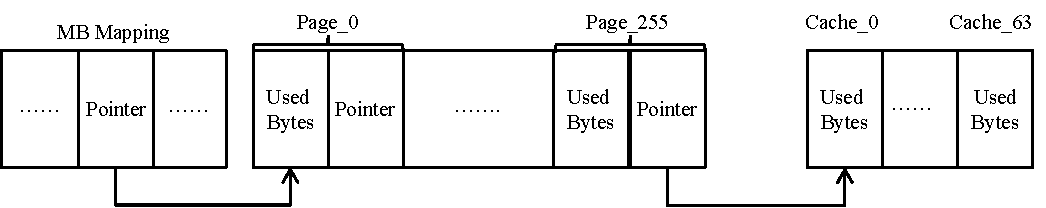
\includegraphics[width=0.9\columnwidth]{figures/lookup}
\caption{Three-level lookup mechanism of \MP{}.\label{fig:lookup}}
\end{figure}

%Note that this design is also efficient in memory consumption. If a range of addresses are not used, then there is no need to allocate physical memory for the corresponding page entries and cache entries. This design is able to adapt to different allocators, where memory mappings of a heap is varied from a few to hundreds of thousands, and these mappings can be scattered along the whole address space of a process. 
%To track valid memory mappings dynamically, \MP{} intercepts memory related system calls inside allocations/deallocations, such as \texttt{sbrk}, \texttt{mmap}, \texttt{munmap}, \texttt{mremap}. 

For false sharing effect, \MP{} focuses on the following aspects: the number of cache lines that has active or passive false sharing, and the number of cache invalidation events. False sharing occurs if two or more threads are accessing different parts of the same cache line. The allocator will introduce false sharing, if an object may share a cache line with others. In particular, the allocator may introduce passive and active false sharing. Passive false sharing is introduced upon deallocations, while active false sharing is introduced during the initial allocations that continuous objects sharing the same cache line are allocated to different threads. Identifying active and passive false sharing is simply based on the definition. However, cache invalidation events are predicted using a simulation-based mechanism, which is borrowed from existing work~\cite{Cheetah}. Basically, \MP{} tracks the last writer (thread id) for each cache line, and then increments the counter of invalidation events if the new writer is different from the last writer. 
%We employ three-level lookup table as discussed above to store the threads information that are allocated from the same cache line. 
In the end, \MP{} reports the percentage of cache invalidation events on cache lines with false sharing issues. 

\MP{} also reports the number of cache contention events on cache lines without active/passive false sharing issues, using the same method. Cache contention events caused by internal-object false sharing or true sharing could also significantly affect the performance, but they cannot be solved with a different memory allocator. However, the reported data could help understand whether an application is running slow or not. Note that \MP{} is not designed to be false/true sharing detection tool. If \MP{} reports a high cache contention rate, users may resort to specific tools to identify specific issues inside the application~\cite{Sheriff, Predator, DBLP:conf/ppopp/ChabbiWL18}. 
   

\begin{comment}


\subsection{Predicting Performance Impact}
\label{sec:predict}

To help users determine whether an allocator is one culprit of the performance issue, \MP{} further predicts the potential performance impact of caused by the allocator. To quantify the impact, \MP{} predicts the potential performance improvement after switching to a target allocator. Currently, we are using TcMalloc as the target allocator, since it has the better overall performance. 

As described above, the allocator could affect the performance of the applications by both application friendliness and memory management overhead. \MP{} only focuses on the latter one, which provides an lower bound on the potential improvement. Basically, \MP{} replaces the runtime of memory management operations with the runtime of the target allocator, and then predicts the reduction of the total runtime. However, the prediction is not   

%For the standard runtime of every memory management operation, \MP{} utilizes the median values collected from a range of applications. Basically, based on our evaluation, the default Linux, TcMalloc, and jemalloc are three best allocators in terms of the performance. Then we choose the best allocator for each application in terms of cycles for each memory management operation, and then select the median value for each operation. Note that there are different choices to choose the standard runtime for every operation, and we only utilizes a simple one to proof the concept. We have thought about that the runtime of a memory management operation can be related with the parallelization and the frequency of allocation. However, it is challenging to build a direct relationship based on our evaluation results. For instance, a serial allocation can also take tens of thousands of cycles. 

To predict the runtime reduction, \MP{} further collects the runtime outside memory management operations with the RDTSC instruction. 
     
	
\end{comment}

\subsection{Predicting Performance Impact}

\label{sec:predict}

\MP{} predicts performance impact of the current allocator. More specifically, it can predict the possible performance improvement if the current allocator is replaced by a target allocator. The prediction is able to predict the slowdown caused by slow memory management operations, but not the slowdown caused by application-friendliness, which is too complicated to predict accurately. For instance, a sampled 22\% cache contention rate of passive false sharing may lead to $38\times$ performance difference of TcMalloc on the \texttt{cache-thrash}, comparing to the default allocator. 

The basic idea of the prediction is to replace the cycles of every memory management operation with the corresponding ones of the target allocator. Currently, the target allocator is TcMalloc, which could be easily changed to any allocator via a configuration file. Note that different types of memory management operations have a vast difference in their cycles, including parallel or serial phases, small or big objects, allocations or deallocations, and re-used or new allocations, as shown in Table~\ref{tbl:metrics}. Therefore, it is important to replace the specified cycle with the corresponding type. The cycles of the target allocator could be manually provided via a configuration file. 

Note that the target allocator may have a different threshold for differentiating small and bit objects, and the performance difference of small and big objects can be as large as $27\times$. Therefore, it is important to differentiate the type of objects correctly. In order to achieve this target, \MP{} reads the configuration file in the initialization phase, and keeps a set of counters to record the number of objects for the target allocator. In the prediction, the counters for the target allocator will be used to compute the runtime for the target allocator. 
%oc, the average cycles of all applications is used. 

 
%\todo{Should we utilize a configuration file to make this functionality flexible? How to design this configuration file? }  
%The prediction will help both allocator designers and normal users. 



\begin{figure}[!ht]
\centering
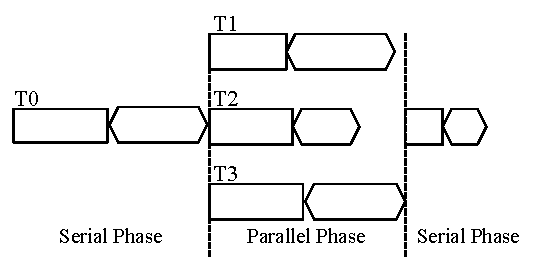
\includegraphics[width=3.2in]{figures/forkjoin}
\caption{Simplified runtime for the prediction, where rectangles indicate the runtime of memory management operations and hexagons are the runtime of others. \label{fig:time}}
\end{figure}

\MP{} is able to predict the performance impact for both single and multi-threaded applications. It simplifies the execution of an application to the model of Figure~\ref{fig:time}. Multithreaded applications have interleaved parallel and serial phases, while there is only one serial phase for single-threaded applications. The prediction is to replace the cycles of each type of memory management operations with the ones in the target allocator, and then computes the total runtime after the replacement. If the predicted runtime is shorter than the original one, \MP{} will predict some performance improvement after the replacement with the target allocator. Otherwise, the target allocator may cause slowdown instead. 

\MP{} makes the prediction of multithreaded applications in the following way. For each parallel phase, it will compute the predicted runtime for every thread separately (treating every thread independently), and then utilize the longest runtime as the runtime for this parallel phase. 
%Second, it will compute the runtime for all threads, but utilizing the average runtime as the prediction for this parallel phase. 
After that, it will compute the total runtime of multiple parallel phases and serial phases. As described in Section~\ref{sec:normalusers},  sometimes \MP{} may have an issue to predict the potential performance improvement, if one thread actually depends on the execution of other threads. 

% How to handle multithreaded applications? 
%\MP{} will automatically detect the critical path for multithreaded applications. For each parallel phase, \MP{} select the thread with most cycles as its critical thread, and calculate the performance improvement of the critical path as the improvement of the whole program. 

%\todo{For applications like \texttt{dedup}, \MP{} will gather the number of pages faults outside allocations for all threads, in order to indicate implicit factors triggered by allocators that could influence the performance}.

 
%The prediction will benefit both allocator developers and normal users. Normal users could base on the prediction to decide whether to change to a new allocator without requiring the actual execution, if \MP{} reports no issues on cache-friendliness. Allocator developers will only check cache-friendliness parameters, if the prediction indicates no performance difference. The evaluation of the prediction can be seen in Section~\ref{}. 

\subsection{Collecting Allocator-Specific Information}
\label{sec:understandingallocators}

\MP{} is designed as a general profiler for different allocators. A configuration file is employed to list the key differences between different allocators, such as the style of the allocator, different types of objects (e.g., small, medium, and big), the sizes of different size classes for small and medium objects, and large object alignment. This configuration file can be provided manually by programmers. Alternatively, \MP{} also provides a pre-run program to automatically determine these details for a given allocator.

In order to identify the style of allocator, the pre-run routine will check whether two subsequent allocations with different sizes (small objects, apparently from different size classes) are satisfied from the same virtual page. 
%If not, then the allocator belongs to a BiBOP-style allocator. Otherwise, it is belonging to the  will belong to the same. 
The information will be used to determine used bytes of cache lines. 
%If they were, then the allocator is a sequential-style allocator, which is similar to the default Linux allocator. Otherwise, the allocator belongs to a BiBOP-style allocator. 

To identify the sizes of the various different size classes, the pre-run routine begins by allocating an object of 8 bytes, and continues to allocate additional objects using a stride increase of 8 bytes each time. The determination of size classes depends on the style of the allocator. For BiBOP-style allocators, an allocation with a different size class will be satisfied from a different bag, located in a different page. For other allocators, we employ the \texttt{malloc\_usable\_size} routine to return the class size. 

%the distance between two contiguously-allocated objects (with distinct sizes) is utilized to determine the size class. As shown in Fig.~\ref{fig:sizeclass}, if the size of $Obj_1$ and $Obj_2$ is the same, judging from the distance of between two continuous objects, then they belong to the same size class. Otherwise, they belong to different size class, such as $Obj_3$ in the figure. By checking the size of two objects belonging to different objects, we could determine the sizes of different size classes.  
\begin{comment}

\begin{figure}[!ht]
\centering
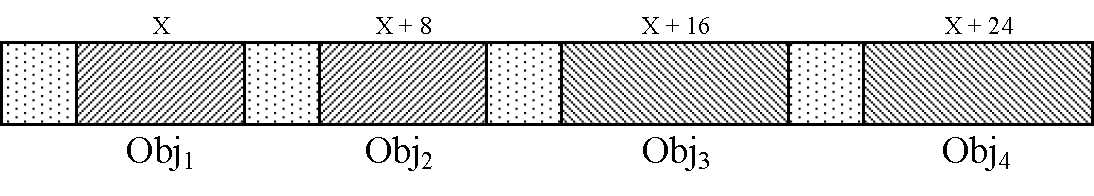
\includegraphics[width=5in]{figures/sequentialclasssize}
\caption{Determining the size class of a sequential allocator by the distance between continuous allocations. \\The boxes with 10\% dotted pattern are the metadata, while the boxes with diagonal stripes\\ are actual heap objects. The number above each box represents the size of the corresponding object. \label{fig:sizeclass}}
\end{figure}
	
\end{comment}

The threshold for big objects are typically detected by checking whether there is an explicit \texttt{mmap} system call upon the allocation request. Typically, most allocators utilize a direct \texttt{mmap} system call to satisfy the allocation of a big object initially. However, this threshold requires manual confirmation. 
